\newpage
\begin{center}
  \textbf{\large 2. Методология}
\end{center}
\refstepcounter{chapter}
\addcontentsline{toc}{chapter}{2. Методология}
\label{method}

\section{Описание метода}
В данном разделе приводится выбор и описание параметров среды для рандомизации, а также методология оценки робастности моделей.

    \subsection{Выбор параметров среды для варьирования}

        Как и в случае доменной рандомизации, задачей является получить достаточно разнообразное распределение вариаций сцен, такое что потенциальная сцена реального мира лежит в рамках этого распределения. Такой подход подразумевает вариацию множества параметров, как физических, так и визуальных. Далее представлено описание 8 выбранных параметров:

        \begin{enumerate}
            \item Параметры объекта манипулирования (ОМ). Объект манипулирования представляет собой целевой объект, с которым робот непосредственное взаимодействует или манипулирует. Вариации ОМ включают: \textbf{цвет ОМ}, \textbf{текстуру ОМ};

            \item Параметры заднего плана. К заднему плану относятся объекты, являющиеся фоновыми на изображениях, доступных агенту, к таким можно отнести стены, стол, источник освещения. Вариации заднего плана включают: \textbf{цвет заднего плана}, \textbf{текстура заднего плана}, \textbf{цвет источника освещения}, \textbf{отвлекающий объект};

            \item Параметры камеры. Вариации камеры включают: \textbf{смещение камеры};

            \item Физические параметры объектов. Вариации физических параметров включают: \textbf{масса объектов}, \textbf{коэффициенты трения объектов}.
        \end{enumerate}

        Выбранные вариации соответствуют потенциальным отличиям между исходным доменном и целевым, а также возмущениям, присущим среде реального мира. 

    \subsection{Процедура варьирования параметров}
         \label{method_randomization}
        Метод варьирования параметров был заимствован также из доменной рандомизации \cite{Peng_2018}. В зависимости от природы параметра было выбрано 3 метода варьирования:

        \begin{enumerate}
            \item \textbf{Непрерывный скалярный случай.} Если параметр принимает некоторое скалярное значение $a \in R$, то его распределение может быть выбрано, как:
            \begin{equation}
                a \sim Uniform(a^* - \varepsilon, a^* + \varepsilon),
            \end{equation}
            где $a^*$ -- значение параметра для исходной, не рандомизированной среды; $\varepsilon$ --  настраиваемый параметр. К параметрам этого типа можно отнести коэффициенты трения, массу. Возможно ситуация, когда значение параметра $a^*$ не известно или не доступно, например, если изучаемая модель была обучена на реальных данных. Для решения этой проблемы есть несколько способов:
                
                \begin{itemize}
                    \item Некоторым образом идентифицировать параметры реального мира, то есть получить оценку интересующего параметра $\hat{a}^*$;
                    \item Зафиксировать приблизительное значение параметра $\hat{a}^*$ и выбрать достаточно большое значение для $\varepsilon$, чтобы распределение вариаций с большей вероятностью покрывало целевой домен.
                \end{itemize}

            \item \textbf{Непрерывный многомерный случай.} Если параметр принимает не скалярное значение, а некоторый вектор размера $n$: $x \in \mathcal{R}^n$, то распределение этого вектора может быть выбрано, как: 

                \begin{equation}
                    x_i \sim \mathrm{Uniform}(x_i^* - \varepsilon, x_i^* + \varepsilon), \quad \forall i \in {1, \dots, n},
                \end{equation}

            где $x_i^*$ -- значение элемента вектора для исходной, не рандомизированной среды; $\varepsilon$ --  настраиваемый параметр, который может быть представлен, как вектор размера 3. Ситуация, когда значения $x_i^*$ неизвестны, решаются аналогично предыдущему случаю.
 
            \item \textbf{Дискретный случай.} Некоторые параметры не могут быть представлены в непрерывном пространстве. Пусть параметр принимает некоторую сущность $x \in \mathcal{X}$, где $\mathcal{X}$ - ограниченное множество допустимых вариаций, тогда распределение для такого параметра может быть представлено в виде:
            
            \begin{equation}
                x \sim \mathrm{Uniform}(\mathcal{X}).
            \end{equation}

            К этому типу параметром, например, относятся текстуры, тогда в качестве $x$ выступает конкретная текстура, то есть изображение, равновероятно выбранная из заданного множества текстур $\mathcal{X}$. 
            
        \end{enumerate}

        Настраиваемые параметры, такие как $\varepsilon$ для непрерывных случаев или элементы множества $\mathcal{X}$ для дискретного случая, зависят от задачи, отличий между исходным и целевым доменами, а также от природы возможных возмущений целевого домена. 
    
        

    \subsection{Метод оценивания робастности моделей}
         \label{method_robust}
        Для получения оценки робастности модели долю успешных эпизодов, полученную в результате эксперимента с исследуемой моделью. 
        
        Процедуру оценивая можно описать следующим образом:

        \begin{enumerate}
            \item Агент выполняет задачу в исходной, не рандомизированной среде. Проводится $N$ экспериментов, доля успешных эпизодов усредняется по количеству эпизодов:

            \begin{equation}
                R_0 = \frac{1}{N} \sum_{i=1}^N \mathbb{I}_{\text{succ}}(E^0_i).
            \end{equation}

            \item Для каждой возможной вариации среды агент аналогично выполняет задачу $N$ экспериментов. Доля успешных эпизодов усредняется по количеству эпизодов:

            \begin{equation}
                R_j = \frac{1}{N} \sum_{i=1}^N \mathbb{I}_{\text{succ}}(E^j_i), \quad \forall j \in {1, \dots, M}.
            \end{equation}

            \item Метрика робастности модели вычисляется как разница между исходной долей успешных эпизодов $p_0$ и долей успешных эпизодов на рандомизированной среде $p_j$:  
            \begin{equation}  
                \Delta R_j = |R_0 - R_j| ,
            \end{equation}  
            где $\Delta R_j$ характеризует робастность модели к $j$-му типу вариаций. Таким образом, чем ближе значение $\Delta R_j$ к $0$, тем устойчивее модель к вариации $j$.

            \item Итоговая метрика робастности модели может быть рассчитана, как усредненное значение $\Delta R_j$ по всем вариациям:

            \begin{equation}  
                \Delta R = \frac{1}{M} \sum_{j=1}^M \Delta R_j ,
            \end{equation}  

            где $\Delta R$ характеризует общую робастность модели, аналогично, чем ближе значение $\Delta R$ к $0$, тем модель робастнее.
            
        \end{enumerate}

    \subsection{Метод оценивания корреляции между эффективностью в симуляторе и в реальности}
       
        Чтобы оценить корреляцию эффективности модели в симуляторе и в реальности, был выбран метод из работы SIMPLER \cite{li24simpler}. Стандартным подходом для определения корреляции между двумя величинами является коэффициент корреляции Пирсона \cite{Pearson}, который может быть рассчитан как:

        \begin{equation}
        r_{XY} = \frac{\text{cov}(X, Y)}{\sigma_X \sigma_Y} = \frac{\sum_{i=1}^n (X_i - \bar{X})(Y_i - \bar{Y})}{\sqrt{\sum_{i=1}^n (X_i - \bar{X})^2} \sqrt{\sum_{i=1}^n (Y_i - \bar{Y})^2}},
        \end{equation}
        где:
        \begin{description}
            \item $X, Y$ -- рассматриваемые выборки
            \item $\text{cov}(X, Y)$ -- ковариация между $X$ и $Y$
            \item $\bar{X}, \bar{Y}$ -- выборочные средние
        \end{description}
        
        Коэффициент Пирсона позволяет оценивать степень линейной зависимости между переменными и применялся в предыдущих исследованиях для оценки качества имитационных оценочных систем \cite{Kadian_2020} путем измерения корреляции между показателями эффективности в реальных условиях и в симуляции. Высокий коэффициент корреляции Пирсона $(\simeq 1)$ свидетельствует о хорошо функционирующей оценочной системе.  Напротив, более низкий коэффициент корреляции может указывать на слабую взаимосвязь между результатами оценки в реальных условиях и в симуляции. 

        При расчете корреляции, эффективность модели в симуляторе рассчитывается, как усредненное значение доли успешных эпизодов по всем вариациям:

        \begin{equation}
            R = \frac{1}{M} \sum_{j=1}^M R_j.
        \end{equation}

        \section{Описание программной реализации}

        В данном разделе описана программная реализация разработанного метода для оценивания робастности модели.

        Предлагаемый метод оценки робастности обученных моделей реализован в виде библиотеки на языке Python на основе фреймворка Isaac Lab \cite{isaaclab}. Isaac Lab представляет собой  модульную платформу для обучения роботов, разработанную с целью упростить исследование методов в робототехнике, таких как обучение с подкреплением и имитационное обучение). Фреймворк является надстройкой над симулятором NVIDIA Isaac Sim \cite{nvidia_isaac_sim}. 

        Isaac Lab предлагает реализацию сред основанных на диспетчерах (англ. Manager-based environments), которые имеют модульную структуру задачи вследствие декомпозиции на отдельно управляемые компоненты. Каждая компонента задачи, такая как вычисление вознаграждений, наблюдений и т.д., может быть определена в виде конфигураций для соответствующего менеджера. Данные менеджеры определяют конфигурируемые функции, ответственные за выполнение специфических вычислений по мере необходимости. Координация совокупности различных менеджеров осуществляется классом Environment, который наследуется от envs.ManagerBasedEnv. Аналогично, все конфигурации должны наследоваться от envs.ManagerBasedEnvCfg.

        Разработанный метод расширяет исходный функционал посредством добавления диспетчера вариаций, полученная архитектура представлена на рис. \ref{fig:arch}. По заданной конфигурации диспетчер вариаций 
        дополняет конфигурацию диспетчера событий, настраивая необходимые рандомизации. Модифицированная конфигурация событий передаётся в класс Environment. Таким образом, разработанный модуль сохраняет модульную структуру исходного фреймворка, что обеспечивает упрощенную интегрируемость в существующее программное обеспечение. На основе описания работы модуля, могут быть выделены следующие ключевые компоненты:
            \begin{itemize}
                \item VariationManagerCfg - конфигурационный класс, определяющий вариаций среды и их параметры. Является уникальным для каждой среды и требует ручной настройки;
                \item VariationManager – диспетчер вариаций, основной модуль, ответственный за управление вариациями среды по заданному конфигурационному файлу VariationManagerCfg;
                \item Validation - класс, отвечающий за проведение экспериментов и обработку результатов.
            \end{itemize}
        
        \begin{figure}
            \begin{center}
                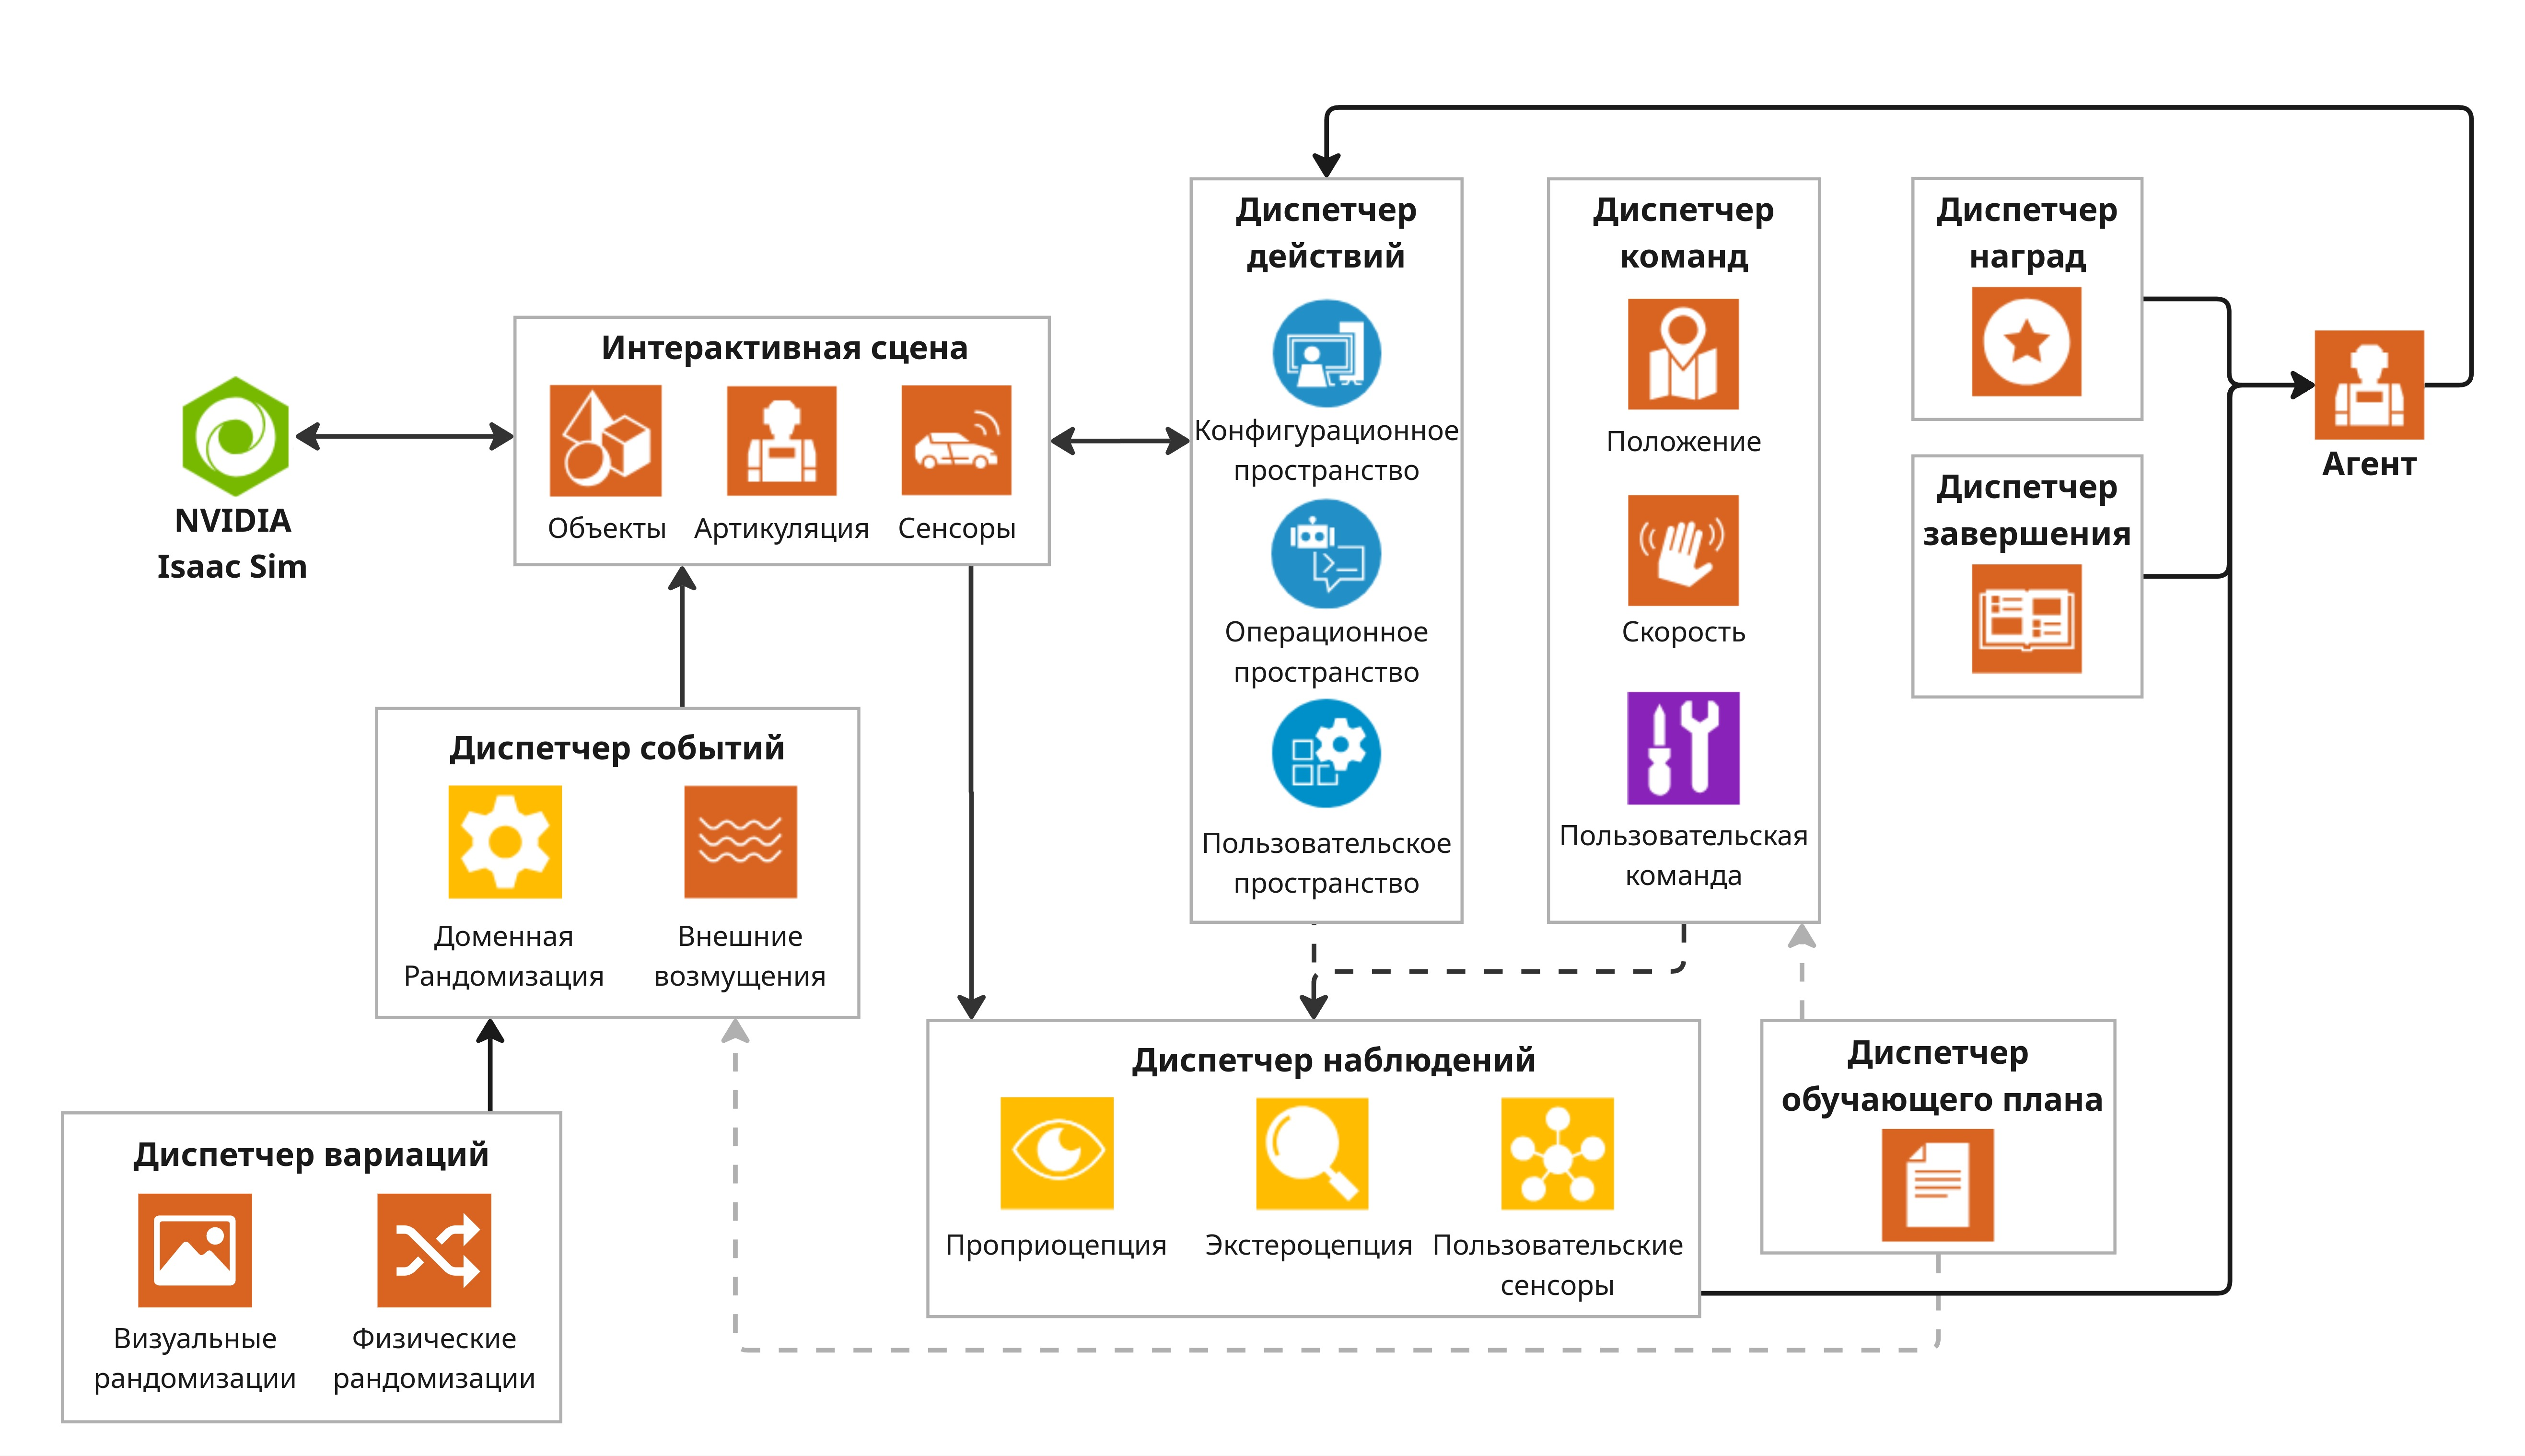
\includegraphics[width=1.0\textwidth]{images/Project Architecture.jpg}
            \caption{Архитектура метода}
            \label{fig:arch}
            \end{center}
        \end{figure}

        \subsection{Модуль варьирования параметров среды}
            Для каждой желаемой вариации создается экземпляр конфигурационного файла VariationCfg, который содержит всю необходимую информацию для применения соответствующей рандомизации, он содержит следующую информацию:

            \begin{itemize}
                \item Название вариации для отражения в отчетных материалах;
                \item Объект функции, которая непосредственно выполняет рандомизацию;
                \item Момент, когда должна применяться рандомизация (при запуске симулятора, в начале нового эпизода и т.д.);
                \item Дополнительные параметры, например, задающие распределение для рандомизированного параметра, распределение задается согласно пункту \ref{method_randomization}.
            \end{itemize} 

            Поля данного класса содержит всю необходимую информацию для создания экземпляров класса EventTerm, которые определяют события среды и регулируются диспетчером событий на верхнем уровне.  
            Чтобы хранить описания всех вариаций, а также настройки диспетчера вариаций, используется класс VariationManagerCfg который определяет конфигурацию для класса VariationManager, непосредственно управляющего всеми вариациями. Перед созданием среды, исходный конфигурационный файл диспетчера событий (EventCfg) передается диспетчеру вариаций, который добавляет экземпляры класса EventTerm, на основе экземпляров класса VariationCfg. Далее, модифицированный конфигурационный файл диспетчера событий передается конструктору среды.

            На нижнем уровне, ключевой является функция, применяющая рандомизацию. Если вариация подразумевает рандомизацию физических параметров, то обновленные параметры среды напрямую записываются в свойства соответствующих объектов и учитываются уже вначале следующего эпизода. Вариация визуальных составляющих является более сложным процессом, ввиду особенностей работы симулятора Isaac Sim. Для реализации подобного функционала в симуляторе представлен фреймворк Omniverse Replicator, предназначенный для разработки пользовательских процессов генерации синтетических данных. Данный фреймворк активно используется при реализации доменной рандомизации в Isaac Sim и поэтому является наиболее уместным для модуля варьирования параметров среды. 
            
        \subsection{Реализация алгоритма оценивания робастности модели}

            Алгоритм оценивания робастности, на основе определенных в \newline VariationManagerCfg вариациях, последовательно применяет их к среде, модифицируя конфигурационный файл диспетчера событий. После применения рандомизаций, исследуемая модель запускается в среде и подсчитываются метрики эффективности, определенные пунктом \ref{method_robust}. Метрики сохраняются в файл, с указанием индекса вариации и измеренным показателем эффективности. Полученные для каждой вариации метрики обрабатываются, и подсчитывается итоговая оценка робастности, аналогично описанию в пункте \ref{method_robust}.
         